\documentclass[12pt,a4]{article}
\usepackage{graphicx}




\usepackage{graphicx,amsmath,amssymb,amsthm, boxedminipage,xcolor,amscd,amsbsy,latexsym,url,bm}

%\usepackage[lined,boxed]{algorithm2e}

\usepackage{algorithm}
\usepackage{algpseudocode}


\newtheorem{theorem}{Theorem}[section]
\newtheorem{proposition}[theorem]{Proposition}
\newtheorem{lemma}[theorem]{Lemma}
\newtheorem{corollary}[theorem]{Corollary}
\newtheorem{definition}[theorem]{Definition}

\newtheorem*{theorem*}{Theorem}
\newtheorem*{lemma*}{Lemma}
\newtheorem*{solution}{Solution}
\newtheorem*{proposition*}{Proposition}


\newtheorem{exercise}[theorem]{Exercise}
\newtheorem{exerciseD}[theorem]{*Exercise}
\newtheorem{exerciseDD}[theorem]{**Exercise}

\let\oldexercise\exercise
\renewcommand{\exercise}{\oldexercise\normalfont}

\let\oldexerciseD\exerciseD
\renewcommand{\exerciseD}{\oldexerciseD\normalfont}

%\let\oldexerciseD\exerciseD
%\renewcommand{\exerciseD}{\oldexerciseD\normalfont}

%\let\oldexerciseDD\exerciseDD
%\renewcommand{\exerciseDD}{\oldexerciseDD\normalfont}

\newcommand{\E}{\mathbb{E}}
%\newcommand{\nth}[1]{#1^{\textsuperscript{th}}}
\newcommand{\scalar}[2]{\ensuremath{\langle #1, #2\rangle}}
\newcommand{\floor}[1]{\left\lfloor #1 \right\rfloor}
\newcommand{\ceil}[1]{\left\lceil #1 \right\rceil}
\newcommand{\norm}[1]{\|#1\|}
\newcommand{\pfrac}[2]{\left(\frac{#1}{#2}\right)}
\newcommand{\nth}[1]{#1^{\textsuperscript{th}}}
\newcommand{\core}{\textnormal{core}}



\newif\ifsolution

\solutionfalse

\newcommand{\answer}[1]{
\ifsolution
{\color{blue} #1}
\else
\fi
}



\newcommand{\poly}{\textnormal{poly}}
\newcommand{\quasipol}{\textnormal{quasipol}}
\newcommand{\ssubexp}{\textnormal{stronglySubExp}}
\newcommand{\wsubexp}{\textnormal{weaklySubExp}}
\newcommand{\simplyexp}{\textnormal{E}}
\newcommand{\expo}{\textnormal{Exp}}



\newcommand{\N}{\mathbb{N}}
\newcommand{\nn}{\mathbb{N}_0^n}
\newcommand{\R}{\mathbb{R}}
\newcommand{\Z}{\mathbb{Z}}


\definecolor{darkgreen}{rgb}{0,0.6,0}

\date{}

\title{
\hbox{  Mathematical Foundations of Computer Science}
  \vspace{3mm}
{\normalsize CS 499,	Shanghai Jiaotong University,  Dominik Scheder\\
%\vspace{3mm}
Spring 2019}
}


\begin{document}

\maketitle

%\begin{quotation}
%  You are welcome to discuss the exercises in the discussion
%  forum. Please take them serious. Doing the exercises is as important
%  than watching the videos.
%
%  I intentionally included very challenging exercises and marked them
%  with one or two ``$*$''. No star means you should be able to solve
%  the exercises without big problems once you have understood
%  the material from the video lecture. One star means it requires 
%  significant additional thinking. Two stars means it is not 
%  unlikely that you will fail to solve them, even once you have understood
%  the material and thought a lot about the exercise. Don't feel bad
%  if you fail. Failure is part of learning.
%
%  This is the first time this course is online. Thus there might be mistakes
%  (typos or more serious conceptual mistakes) in the exercises. I will be 
%  grateful if you point them out to me!
%\end{quotation}




\setcounter{section}{0}


\begin{center}
  \large\textbf{Group: navigator} 
\end{center}
\begin{center}
  \begin{tabular}{rl}
 Xu Huan  & 517021910724 \\
 Tianyao Shi     &     517021910623 \\
Chenxiao Yang    &    517021910540  \\
Jiaqi  Zeng      &     517021910882  \\
  \end{tabular}
\end{center}

\newpage 
\section{Broken Chessboard and Jumping With Coins}

\subsection{Tiling a Damaged Checkerboard}

In the video lecture you have seen a proof that one cannot
tile the ``damaged'' $8 \times 8$ checkerboard with domino stones:
\begin{center}
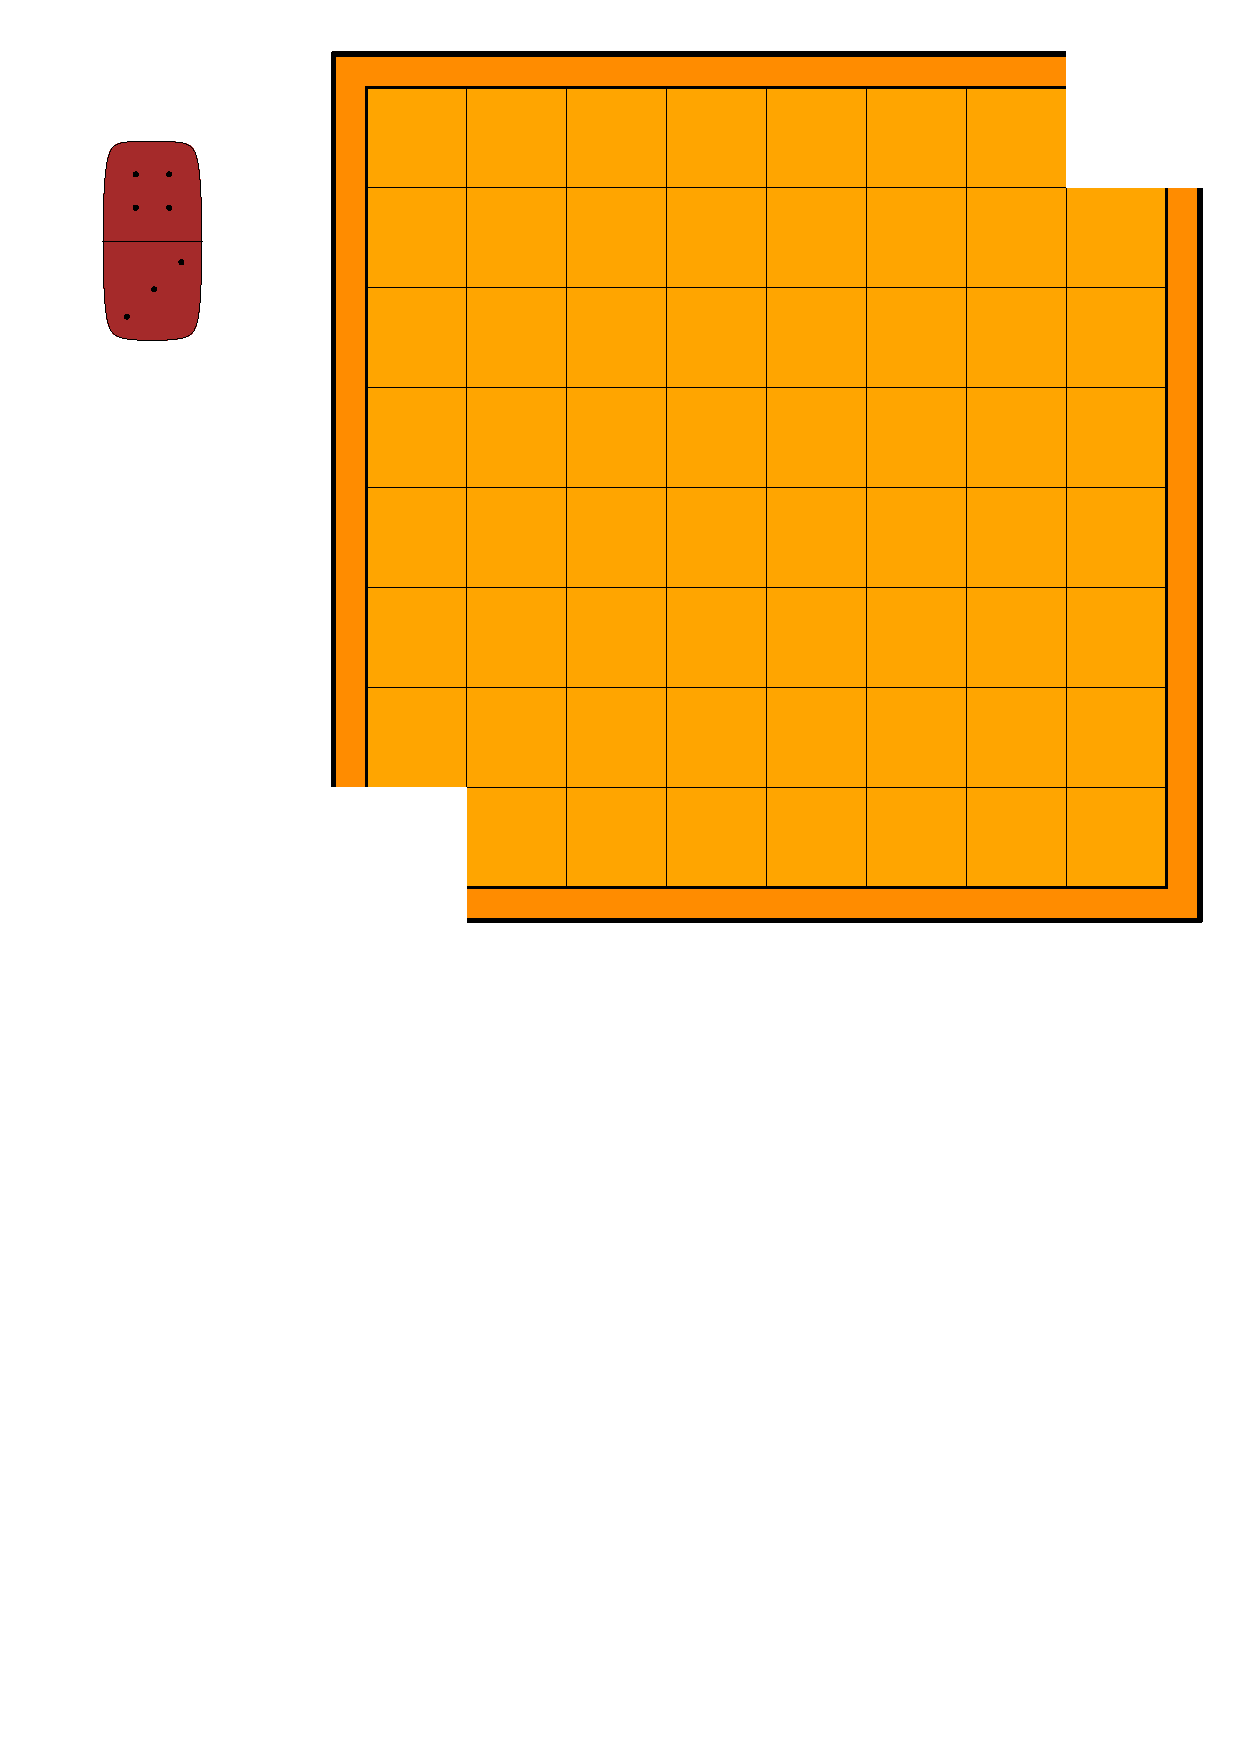
\includegraphics[width=0.4\textwidth]{figures/checkerboard-without-corners.pdf}
\end{center}

\begin{exercise}
  Re-write the proof in your own way,  using simple English sentences.
\end{exercise}

\begin{proof}
  Color the checkboard with black and white.

  Observe that one domino stone on the checkerboard must occupy 1 black check and 1 white check.

  Since the checkerboard without corners only has 30 black checks and 32 white checks, obviously, the original statement is not established.
  \begin{center}
    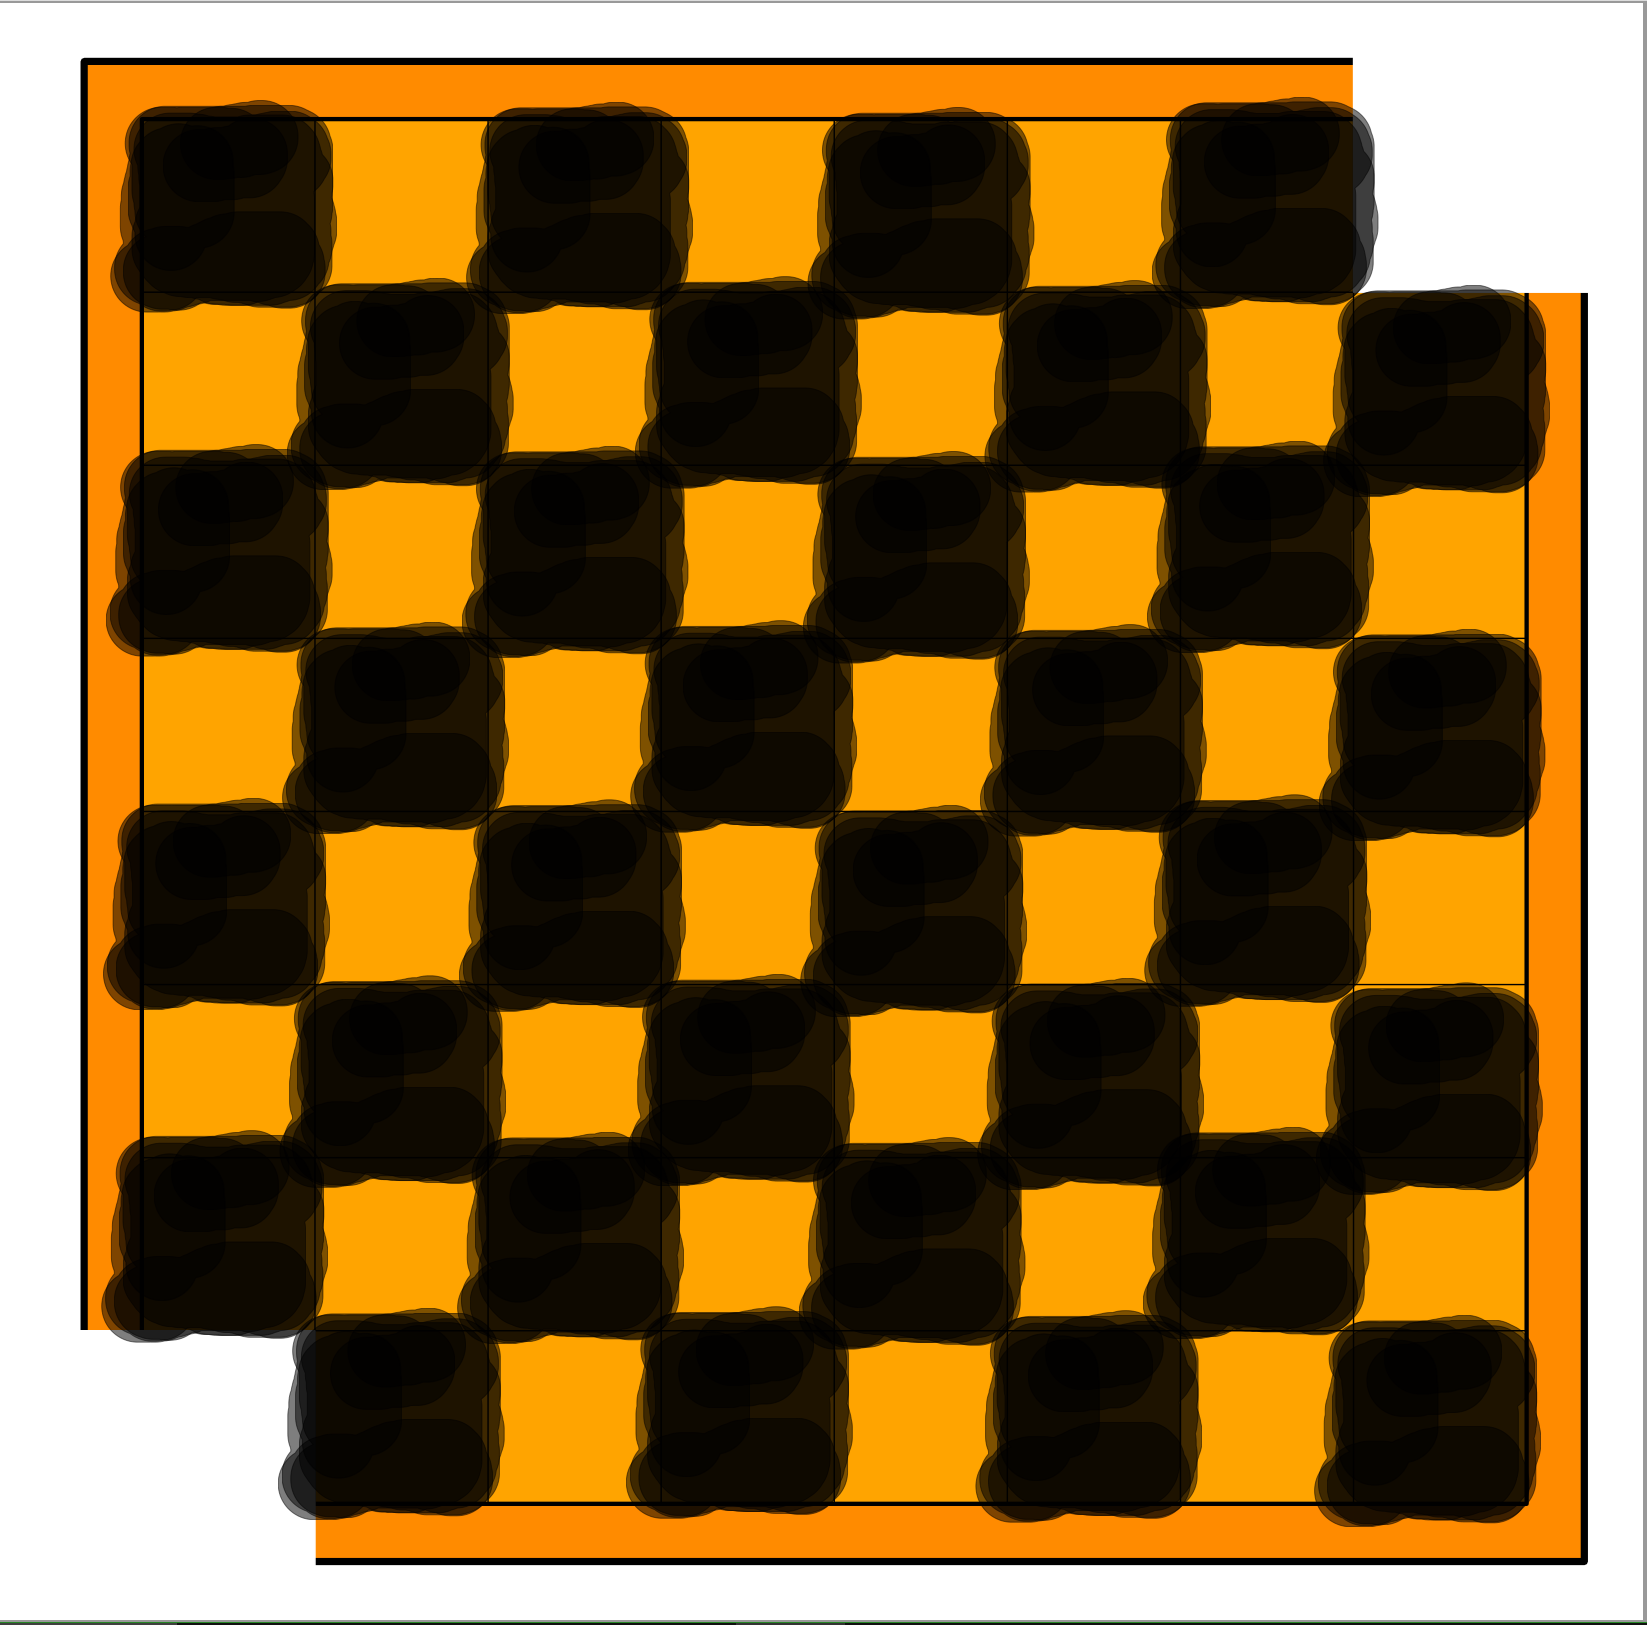
\includegraphics[width=0.4\textwidth]{figures/checkerboard-without-corners-colored.png}
  \end{center}
\end{proof}

\begin{exercise}
  Look at the seriously damaged $8 \times 8$ checkerboard. For convenience
  I already colored it black and white (or rather black and beige):
  \begin{center}
    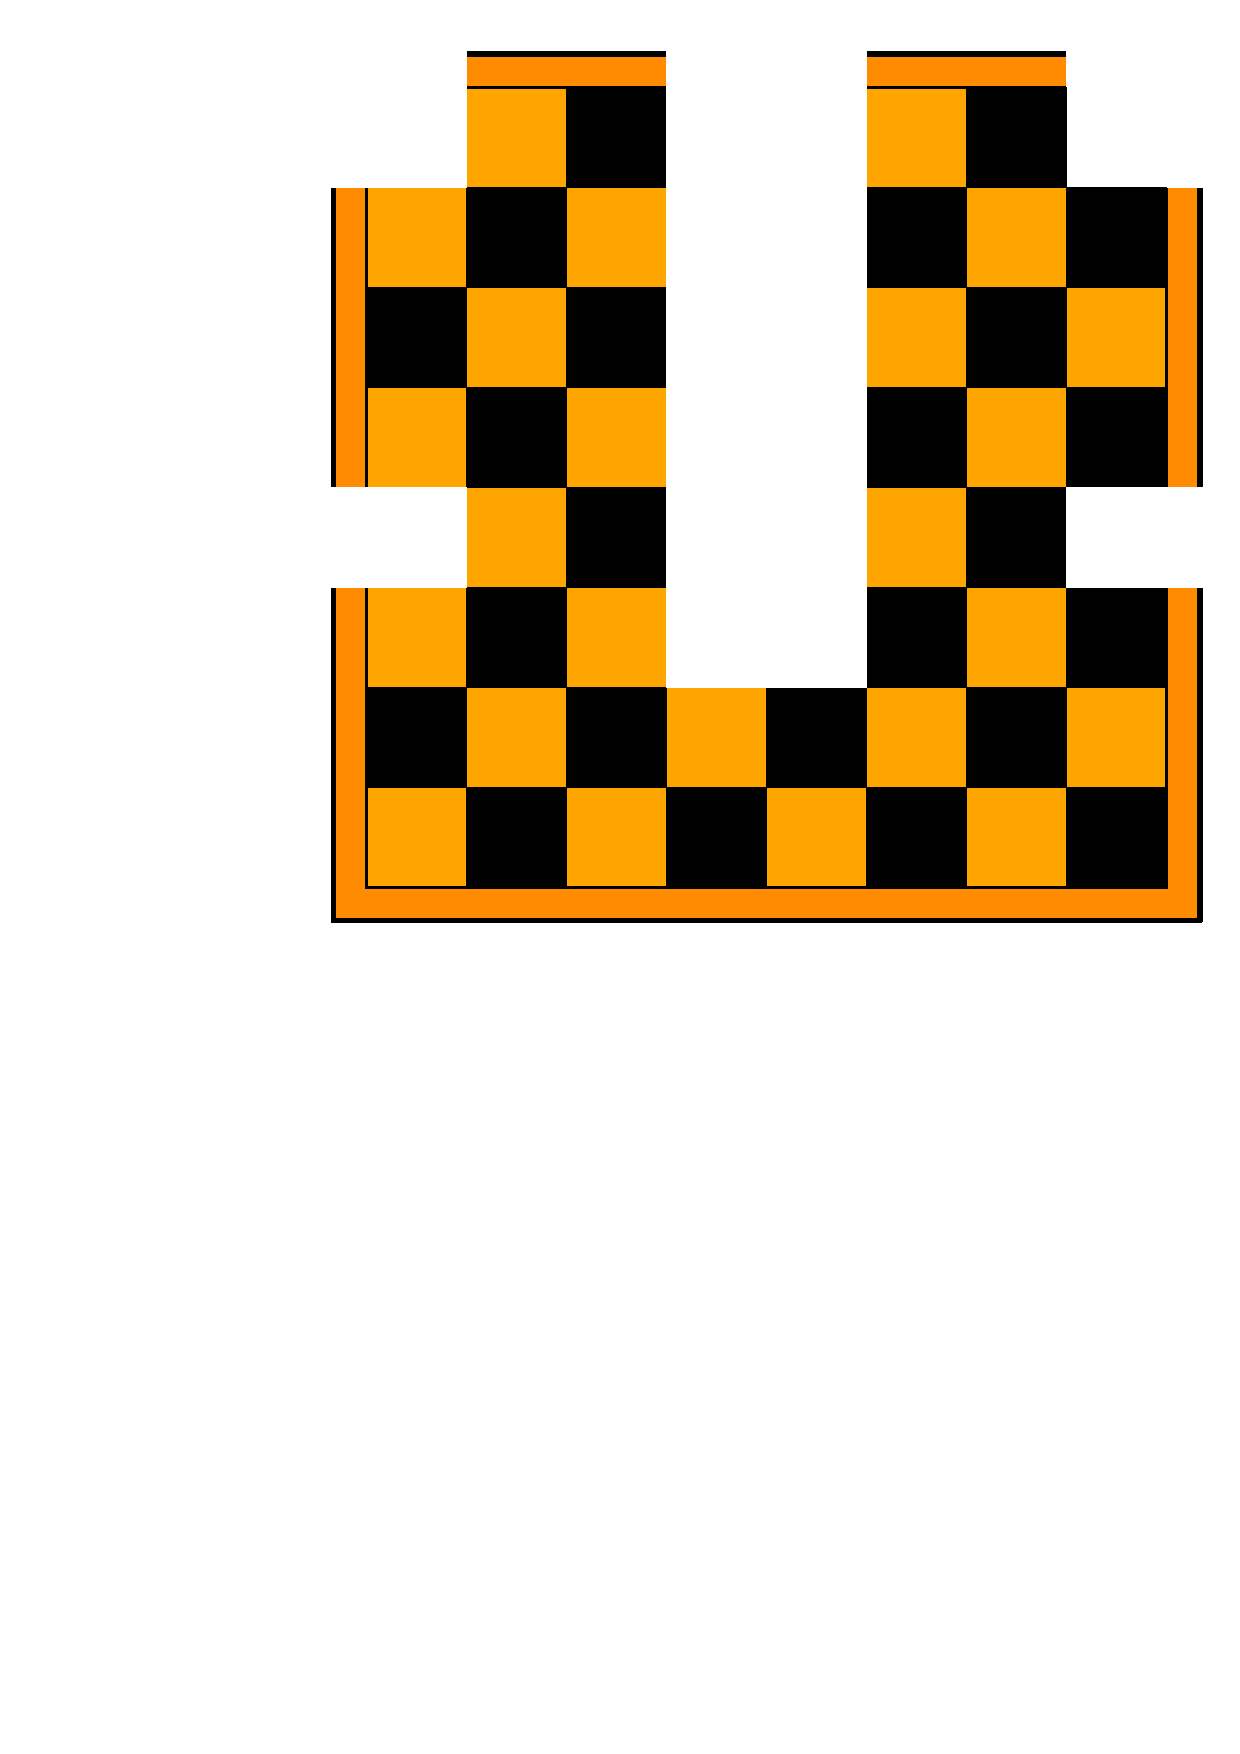
\includegraphics[width=0.4\textwidth]{figures/checkerboard-8x8-damaged.pdf}
  \end{center}
  Try to tile it with domino stones and you will fail. However, since
  there are $24$ black and $24$ beige squares, the simple argument from
  the lecture will fail. 

  Prove that the above board cannot be tiled. Try to find a short and simple
  argument! 
\end{exercise}
  
\begin{proof}
  Observe the area where the checks are numbered in the checkerboard.

  Notice that there are 12 white checks and 11 black checks.

  Since one domino stone must occupy 1 black check and 1 white check, a black check adjacent to this area is needed.

  However, obviously, there is no black check statisfying that requirement.

  Therefore, the original statement is not established.
  \begin{center}
    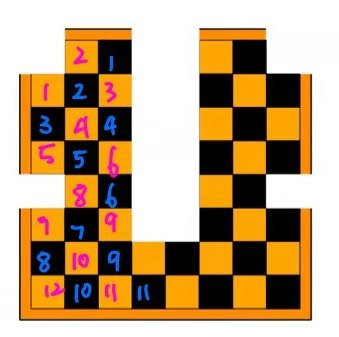
\includegraphics[width=0.4\textwidth]{figures/checkerboard-damaged-numbered.jpg}
  \end{center}
\end{proof}

\subsection{Jumping with Coins}

This is simply a reminder of the exercises I posed in the video lecture.
For details, refer to the video.

\textbf{Remark.} The following exercises are of different levels
of difficulty, but they all have a very simple proof (altough the proof
might not be easy to find).

\begin{exercise}
  You jump around with two coins. Show that you cannot increase the distance between
  the two coins. 
  \begin{center}
    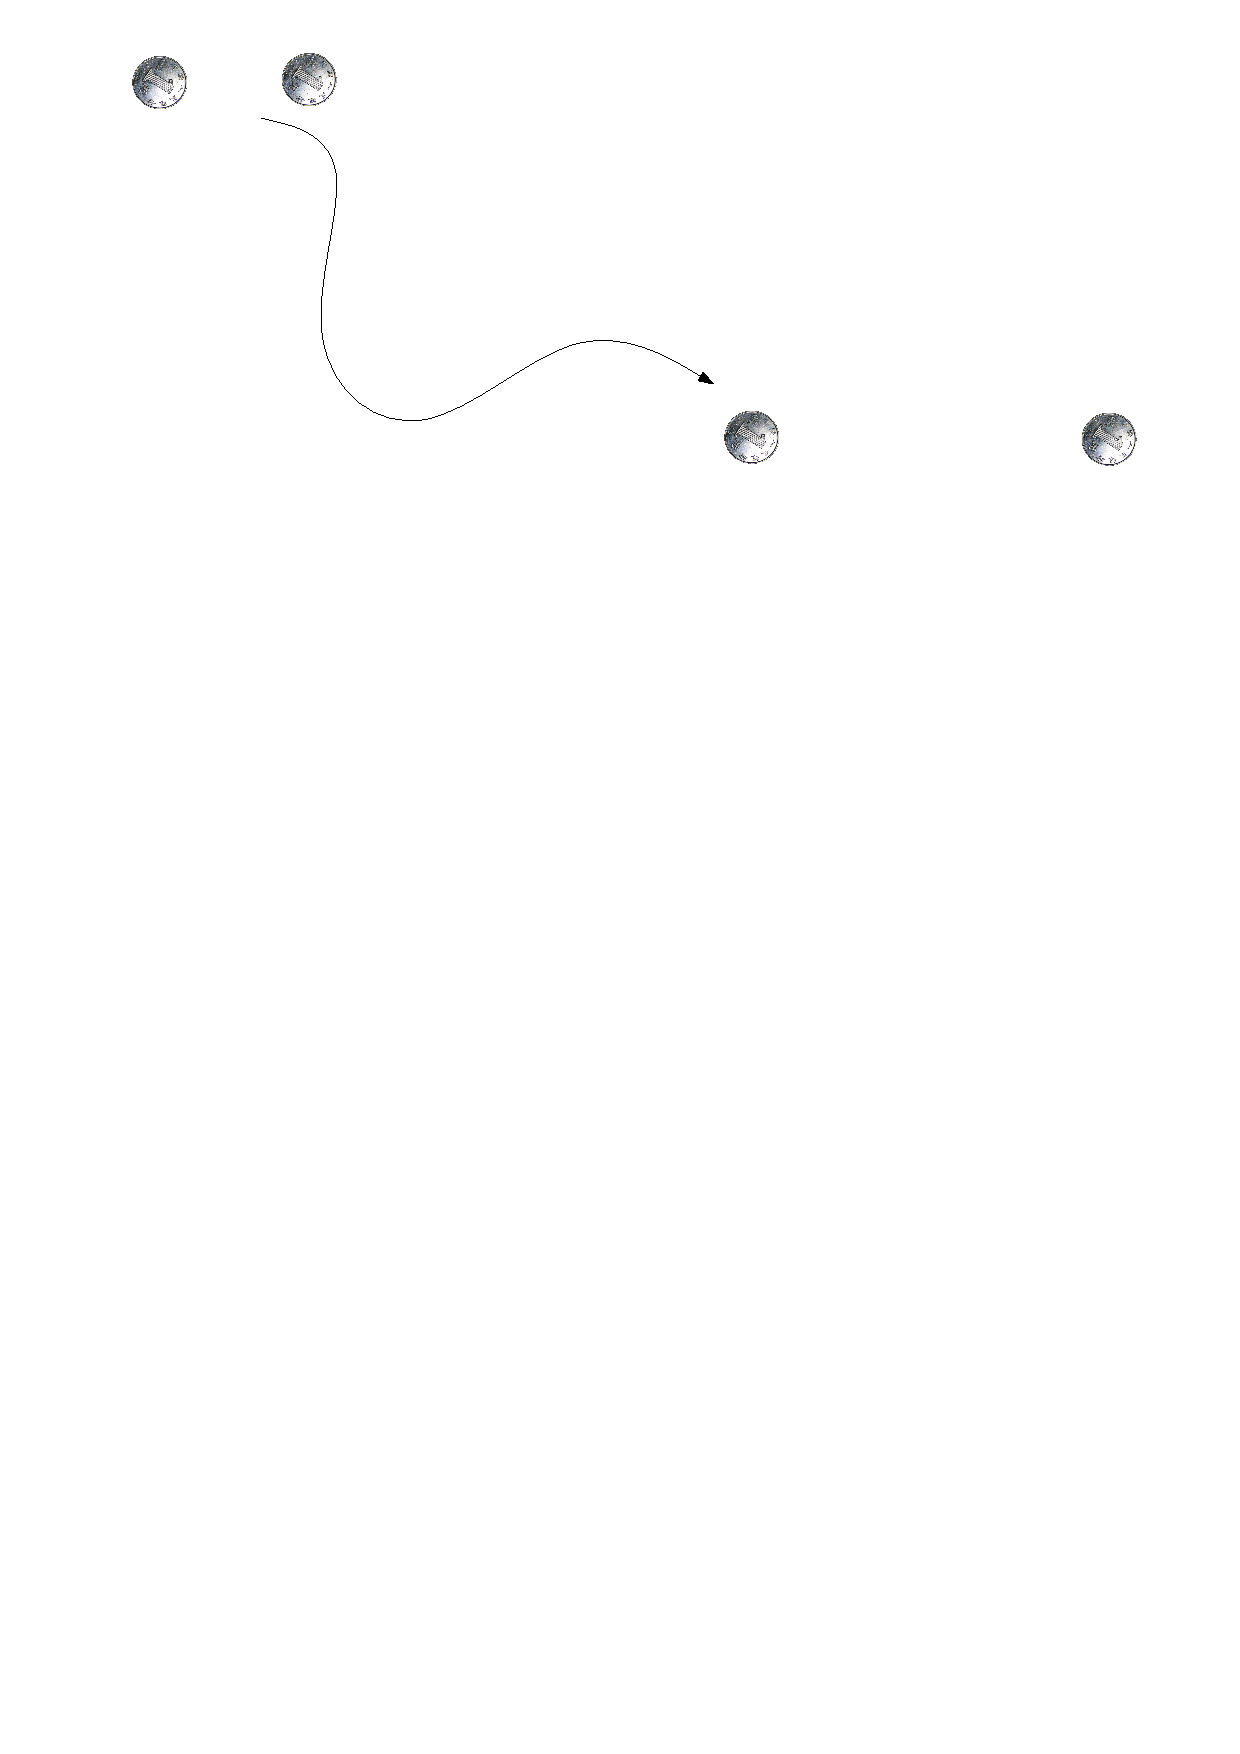
\includegraphics[width=0.4\textwidth]{figures/coins-2.pdf}
  \end{center}
\end{exercise}

\begin{proof}
  According to the rules, in every move, one coin is still and another do symmetric operation. In Figure \ref{two}, $d1=d2$, so we cannot increase the distance between the two coins.
  \begin{figure}[htbp]
  \begin{center}
    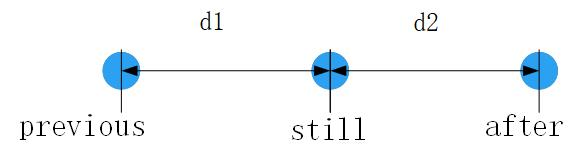
\includegraphics[width=0.4\textwidth]{figures/two.jpg}
    \caption{Figure for two coins}\label{two}
  \end{center}
\end{figure}
\end{proof}


\begin{exercise}
  You jump around with three coins. Show that you cannot start with an equilateral
  triangle and end up with a bigger equilateral triangle. Give a simple proof!
  \begin{center}
    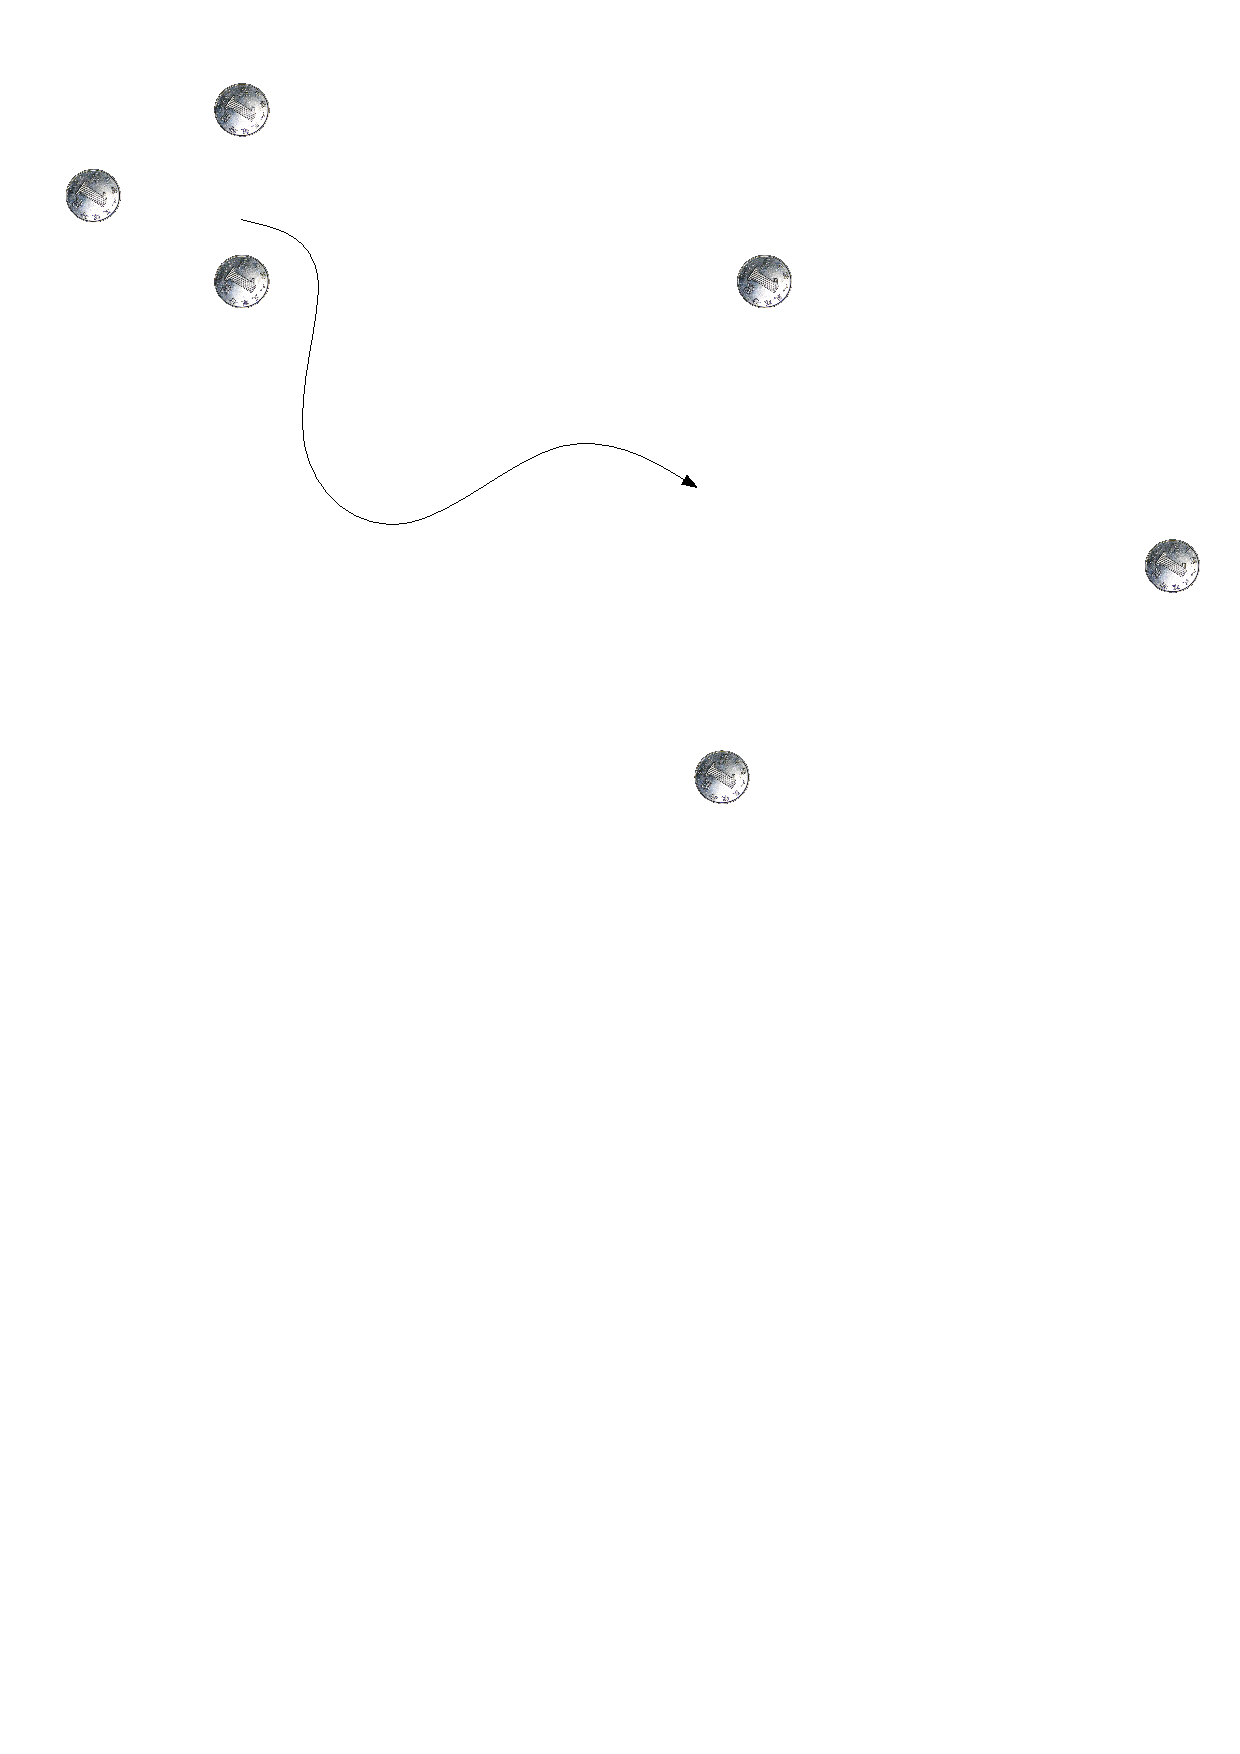
\includegraphics[width=0.5\textwidth]{figures/coins-3.pdf}
  \end{center}
\end{exercise}

\begin{proof}
  In every move, as we have prove in Exercise 1.3, we cannot increase the distance between the two coins. We can regard it as the immutability of the triangle's bottom line. Meanwhile, we can see the height is also constant within a move as Figure \ref{three} shows. Therefore, using the formula $area=(bottom line \times height)/2$, we get that the area of triangle is constant. So we cannot start with an equilateral
  triangle and end up with a bigger equilateral triangle.
  \begin{figure}
  \begin{center}
    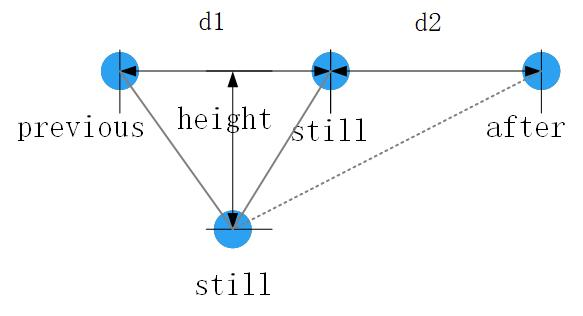
\includegraphics[width=0.5\textwidth]{figures/three.jpg}
    \caption{Figure for three coins}\label{three}
  \end{center}
\end{figure}
\end{proof}

You jump around with four coins which in the beginning form a square of side length $1$. 

\begin{center}
  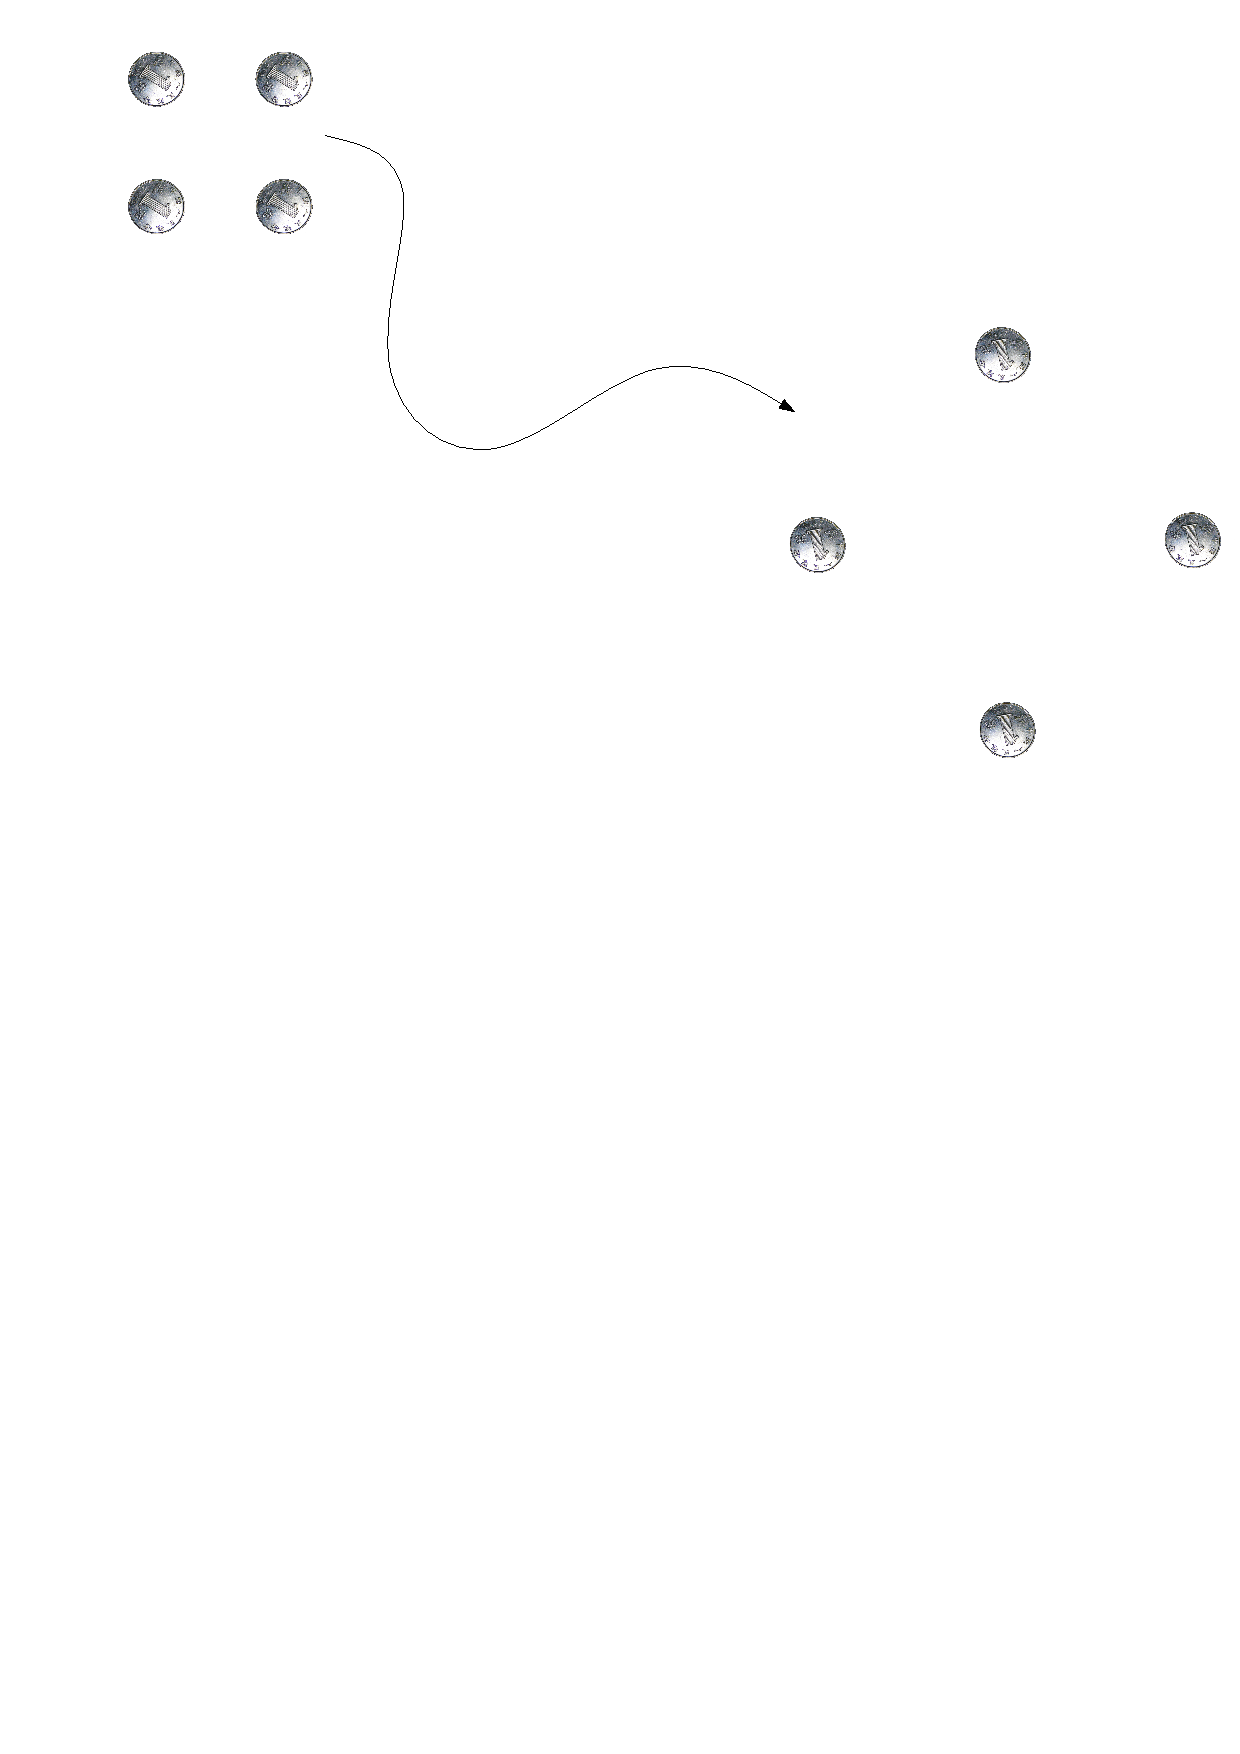
\includegraphics[width=0.5\textwidth]{figures/coins-4.pdf}
\end{center}

\begin{exercise}
  Show that you cannot form a square of side length $2$.
\end{exercise}

\begin{proof}
  We establish a coordinate system as Figure \ref{four1} shows. In Figure \ref{four1} we can give each coin of the black square a coordinate, which is $(0,0), (0,1), (1,0), (1,1)$ respectively. In every moves, coins need to move $2n$ units in both $x$ direction and $y$ direction ($n=0, 1, 2, \cdot\cdot\cdot$). Therefore, the coin with $(0,0)$ coordinate can only move to the location whose abscissa and ordinate are both even numbers. Similarly, the coin with $(0,1)$ coordinate can only move to the location whose abscissa is even and ordinate is odd. The coin with $(1,0)$ coordinate can only move to the location whose abscissa is odd and ordinate is even. The coin with $(1,1)$ coordinate can only move to the location whose abscissa and ordinate are odd numbers. This means that two coins cannot have the same parities in their abscissas and ordinates. However, in a square of side length $2$, all four coins have the same parities in their abscissas and ordinates. Therefore, we cannot form a square of side length 2.


  \begin{figure}
  \begin{center}
    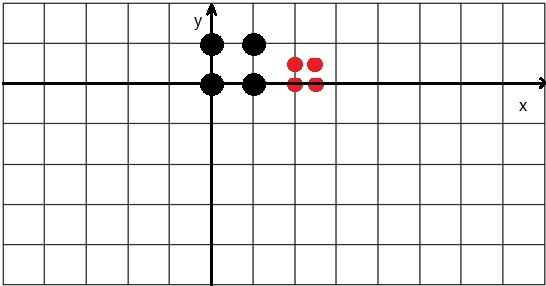
\includegraphics[width=0.6\textwidth]{figures/four1.jpg}
  \end{center}
  \caption{Figure for four coins}\label{four1}
\end{figure}
\end{proof}

\begin{exercise}
  Show that you cannot achieve a position in which two coins are at the same position.
\end{exercise}

\begin{proof}

  %We establish a coordinate system as Figure \ref{four1} shows. In Figure \ref{four1} we can give each coin of the black square a coordinate, which are $(0,0), (0,1), (1,0), (1,1)$. In every moves, coins need to move $2n$ units in both $x$ direction and $y$ direction ($n=0, 1, 2, \cdot\cdot\cdot$). Therefore, the coin with $(0,0)$ coordinate can only move to the location whose abscissa and ordinate are both even numbers. Similarly, the coin with $(0,1)$ coordinate can only move to the location whose abscissa is even and ordinate is odd. The coin with $(1,0)$ coordinate can only move to the location whose abscissa is odd and ordinate is even. The coin with $(1,1)$ coordinate can only move to the location whose abscissa and ordinate are odd numbers. %
  This proof is similar to the proof of Exercise 1.5. From the proof of Exercise 1.5, we conclude that two coins cannot have the same parities in their abscissas and ordinates. This alse means we cannot achieve a position in which two coins are at the same position.

\end{proof}


\begin{exercise}
  Show that you cannot form a larger square.
\end{exercise}

\begin{proof}
  According to the rule, we can see the every moves are reversible. We can form a checkerboard and put each coin at a point. If we want to form a smaller square, the square may be like the red one in Figure \ref{four1}. However, in each move, the coin will fall on one intersection and it is impossible to fall between two adjacent intersections. Therefore, we cannot narrow a square. Zooming in on a square is a reversible operation of narrowing a square. If we cannot make a square smaller, it is also impossible to form a larger square.

\end{proof}




\section{Exclusion-Inclusion}

\subsection{Sets}


\begin{exercise}
  Let $A,B,C$ be finite sets.
  \begin{enumerate}
  \item Prove that $|A \cup B| = |A| + |B| - |A \cap B|$.
  \begin{proof}
    
      \begin{figure}[h]
        \centering
        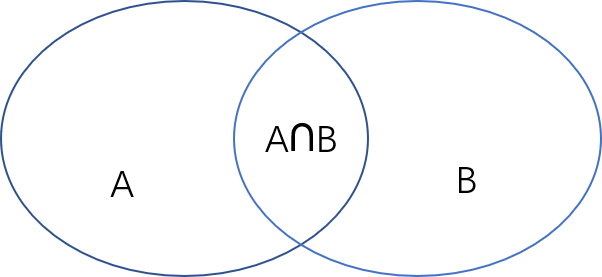
\includegraphics[width=0.5\textwidth]{figures/Venn1.png}
        \caption{Venn figure of the two-set case.}  \label{fig:venn}
      
      \end{figure}
      
  As is shown in Figure~\ref{fig:venn}, when we want the size of $A\cup B$, we add $|A|$ and $|B|$ up. Then we find that the part $A\cap B$ in between is added twice, so we subtract it once, so that each element in $A\cup B$ is and is only counted once. Therefore, we have $|A \cup B| = |A| + |B| - |A \cap B|$.
  \end{proof}
  \item What about $|A \cup B \cup C|$? Find a formula in terms 
  of pairwise and three-wise intersections.
  \begin{proof}[Solution:]
    Using the same method in the former question, we have $|A \cup B\cup C| = |A| + |B|+|C| - |A \cap B|-|B\cap C|-|C\cap A|+|A\cap B\cap C|$.
  \end{proof}
  \item What about $|A \cup B \cup C \cup D|$? Find a formula in terms of 
  pairwise, three-wise, and four-wise intersections.
\begin{proof}[Solution:]
    Using the same method in the former question, we have $|A \cup B\cup C\cup D| = |A| + |B|+|C|+|D| - |A \cap B|-|B\cap C|-|C\cap A|-|A \cap D|-|B\cap D|-|C\cap D|+|A\cap B\cap C|+|A\cap B\cap D|+|A\cap C \cap D|+|B \cap C \cap D|-|A\cap B\cap C\cap D|$.
  \end{proof}
  \label{in-ex-three}
  \end{enumerate}
  \label{exercise-inclusion-exclusion}
\end{exercise}

\begin{exercise}[The Exclusion-Inclusion Formula]
  Maybe you have noticed a pattern. Find a general formula, i.e., for
  $|A_1 \cup \dots \cup A_n|$ in terms of the size of intersections 
  $A_I :=  \bigcap_{i \in I} A_i$.
  
  \begin{proof}[Solution:]
    The general formula takes the following shape: 
  \begin{align*}  
    &|A_1 \cup \dots \cup A_n| = \\
    &\sum_{1\leq i\leq n}|A_i| -\sum_{1\leq i<j\leq n}|A_i \cap A_j|+\sum_{1\leq i<j<k\leq n}|A_i\cap A_j\cap A_k|+\dots +(-1)^{n-1}|A_1\cap A_2\cap \dots\cap A_n|.
    \end{align*}
  \end{proof}
\end{exercise}


\begin{exercise}
  Justify the formula you found in the previous exercise. 
  \textbf{Hint.} There is a proof using induction on $n$. \textbf{Hint.} There is 
  a proof that does not need induction on $n$.
  
  As the hint goes, here we present two kinds of different proofs. The first one uses induction while the second one does not.
  \begin{proof}
    We use mathematical induction to prove the equation beyond. 
    
    When $n=2$, as is proved in Exercise~\ref{exercise-inclusion-exclusion}, the equation holds.
    
    Suppose that the equation is correct when $n=s(s\geq2)$. When $n=s+1$, we have
    \begin{align*}
      &|A_1 \cup \dots \cup A_n| = |A_1 \cup \dots \cup A_s\cup A_{s+1}|\\
      =&|A_1 \cup \dots \cup A_s|+|A_{s+1}|-|(A_1 \cup \dots \cup A_s)\cap A_{s+1} |  \\
      =&\sum_{1\leq i\leq s}|A_i| -\sum_{1\leq i<j\leq s}|A_i \cap A_j|+\sum_{1\leq i<j<k\leq s}|A_i\cap A_j\cap A_k|\\
       &+\dots +(-1)^{s-1}|A_1\cap A_2\cap \dots\cap A_s|+|A_{s+1}|-\left|\bigcup_{i=1}^s(A_i\cap A_{s+1})\right|\\
       =&\sum_{1\leq i\leq s+1}|A_i| -\sum_{1\leq i<j\leq s}|A_i \cap A_j|+\sum_{1\leq i<j<k\leq s}|A_i\cap A_j\cap A_k|\\
       &+\dots +(-1)^{s-1}|A_1\cap A_2\cap \dots\cap A_s|-\sum_{1\leq i\leq s}|A_i \cap A_{s+1}|\\
       &+ \sum_{1\leq i<j\leq s}|(A_i\cap A_{s+1}) \cap (A_j\cap A_{s+1})|
       - \sum_{1\leq i<j<k\leq s}|(A_i\cap A_{s+1})\cap|(A_j\cap A_{s+1})\cap|(A_k\cap A_{s+1})|\\
       &+\dots-(-1)^{s-2}\sum_{1\leq i_1<\dots<i_{s-1}\leq s}|A_{i_1}\cap \dots\cap A_{i_{s-1}}\cap A_{s+1}|-(-1)^{s-1}\left|\bigcap_{i=1}^s(A_i\cap A_{s+1})\right|\\
       =&\sum_{1\leq i\leq s+1}|A_i| -\sum_{1\leq i<j\leq s+1}|A_i \cap A_j|+\sum_{1\leq i<j<k\leq s+1}|A_i\cap A_j\cap A_k|\\
       &+\dots+(-1)^{s-1}\sum_{1\leq i_1<\dots<i_s\leq s+1}|A_{i_1}\cap \dots\cap A_{i_s}|+(-1)^s\left|\bigcap_{i=1}^{s+1}A_i\right|.
    \end{align*}
    That is to say, when $n=s+1$, the equation holds. Therefore, the formula is true for every $n\geq2$.
  \end{proof}

\begin{proof}
  For any $x\in A_1\cup A_2\cup\dots\cup A_n$, assume that there are $m$ different sets in $A_1$, $A_2$, $\dots$, $A_n$ that contain element $x$, where $1\leq m\leq n$. Moreover, $A_i\cap A_j$ contains $x$ if and only if both $A_i$ and $A_j$ contain $x$. Therefore, there are ${m \choose 2}$ pairwise intersections in all that contain $x$.
  
  Likewise, there are ${m \choose 3}$ three-wise intersections in all that contain $x$. In general, there are ${m \choose k}$ k-wise intersections in all that contain $x$, where $1\leq k\leq m$.
  According to Binomial theorem, we have 
  $$
  0=(1-1)^m=1-m+{m \choose 2}-{m \choose 3}+\dots+(-1)^{m}{m \choose m}
  $$
  Therefore, in the right side of the equation the time $x$ is counted can be derived as
  $$
  m-{m \choose 2}+{m \choose 3}-\dots+(-1)^{m-1}{m \choose m}=1.
  $$
  That is to say, every $x\in A_1\cup A_2\cup\dots\cup A_n$ is and is only counted once according to the formula, for which the formula is correct.
\end{proof}
\end{exercise}

\section{Feasible Intersection Patterns}


\begin{exercise}
 Find sets $A_1,A_2,A_3,A_4$ such that all pairwise intersections have size $3$
 and all three-wise intersections have size $1$. Formally,
 \begin{enumerate}
 \item $|A_i \cap A_j| = 3$ for all $\{i,j\} \in { [4] \choose 2}$,
 \item $|A_i \cap A_j \cap A_k| = 1$ for all $\{i,j,k\} \in { [4] \choose 3}$.
 \end{enumerate}
 \label{exercise-feasible-4}
\end{exercise}
 
\begin{proof}[Solution:]
  Construct sets $A_1,A_2,A_3,A_4$:

  $A_1 = \{a,c,d,e,f,g\}$;  $A_2 = \{a,b,d,e,h,i\}$;

  $A_3 = \{a,b,c,f,h,j\}$;  $A_4 = \{b,c,d,g,i,j\}$;

  $A_1 \cap A_2 = \{a,d,e\}$; $A_1 \cap A_3 = \{a,c,f\}$;

  $A_1 \cap A_4 = \{c,d,g\}$; $A_2 \cap A_3 = \{a,b,h\}$;

  $A_2 \cap A_4 = \{b,d,i\}$; $A_3 \cap A_4 = \{b,c,j\}$;

  $A_1 \cap A_2 \cap A_3 = \{a\}$; $A_2 \cap A_3 \cap A_4 = \{b\}$;

  $A_1 \cap A_3 \cap A_4 = \{c\}$; $A_1 \cap A_2 \cap A_4 = \{d\}$.

\end{proof}


\begin{exercise}
  Show that if we insist that $|A_i| = 5$ for all $i$, then the task from the above exercise cannot be 
  solved.
\end{exercise}

\begin{proof}
  Use the formula mentioned in the previous exercise, 
  $$|\bigcup\limits_{i=1}^4{A_i}| = \sum\limits_{i=1}^4{|A_i|} - \sum\limits_{1\le i < j \le 4}{|A_i \cap A_j|} + \sum\limits_{1\le i < j < k \le 4}{|A_i \cap A_j \cap A_k|} - |\bigcap\limits_{k=1}^4{A_k}|$$

  $= 4 \times 5 - 6 \times 3 + 4 \times 1 - |\bigcap\limits_{k=1}^4{A_k}|$

  $= 6 - |\bigcap\limits_{k=1}^4{A_k}|$

  Since $\bigcap\limits_{k=1}^4{A_k} \subset \bigcap\limits_{1 \le i \le 4}^3{A_i}$, $|\bigcap\limits_{k=1}^4{A_k}| \le |\bigcap\limits_{1 \le i \le 4}^3{A_i}| = 1$.

  Case 1. Assume that $|\bigcap\limits_{k=1}^4{A_k}| = 1$. Then $|\bigcup\limits_{i=1}^4{A_i}| = 5$, which means $A_1,A_2,A_3,A_4$ are all the same, contradicting the original statement.

  Case 2. Assume that $|\bigcap\limits_{k=1}^4{A_k}| = 0$. Then $|\bigcup\limits_{i=1}^4{A_i}| = 6$.

  Suppose that $\bigcup\limits_{i=1}^4{A_i} = \{a,b,c,d,e,f\}$. Without loss of generality, we can randomly get rid of 1 element of $\bigcup\limits_{i=1}^4{A_i}$ to construct $A_i$.

  For example, for $A_1$, get rid of a. Then $A_1 = \{b,c,d,e,f\}$.

  By that analogy, $A_2 = \{a,c,d,e,f\}, A_3 = \{a,b,d,e,f\}, A_4 = \{a,b,c,e,f\}$.

  Notice that $|\bigcap\limits_{i=1}^4{A_i}| = 2$, which contradicts the assumption. Thus, this case is not esatablished.

  Therefore, the original statement is false.


\end{proof}

In the spirit of the previous questions, let us call a sequence
$(a_1, a_2, \dots, a_n) \in \N_0$ {\em feasible} if there are sets
$A_1,\dots,A_n$ such that all $k$-wise intersections have size $a_k$.
That is, $|A_i| = a_1$ for all $i$, $|A_i \cap A_j| = a_2$ for all $i \ne j$ and so on.
The previous exercise would thus state that $(5,3,1,0)$ is not feasible, but $(6,3,1,0)$ is, as 
one solution of Exercise~\ref{exercise-feasible-4} shows.

\begin{exerciseD}
 Suppose I give you a sequence $(a_1,\dots,a_n)$. Find a way to determine
 whether such a sequence is feasible or not.
\end{exerciseD}
 
Since this exercise might be too difficult, so I will talk about it in our Thursday class and
break it into more manageable parts.

\begin{proof}[Solution:]
  There are totally n finite sets $A_1,\dots,A_n$. If we draw a Venn diagram, there should be $2^n-1$ regions in it. And we call each region as an \textbf{Atomic Set}. Then, we assign a n-bits binary code to each atomic set, like the figure showed below:
  \begin{center}
      
\includegraphics[width=0.4\textwidth]{figures/venn2.png}
    \end{center}
    We denote the atomic set as $S_{100}$, if it contains $A_1$ but doesn't contain $A_2$ and $A_3$ (in this case n=3). $S_{000}$ is neglected since it is not related to the problem.

    The element number of each atomic set is treated as an unknown variable, so there are totally $2^n-1$ variables. Also, given $(a_1,\dots,a_n)$, we can list $2^n-1$ equations which are linear irrelevant (${n \choose 1}+{n \choose 2}+\dots+{n \choose n}=2^n-1$). For example, when n=3, there are 7 equations:
    \begin{equation}
    \begin{split}
    &a_3=|S_{111}|\\
        &a_2=|S_{111}|+|S_{011}|\\
    &a_2=|S_{111}|+|S_{101}|\\
    &a_2=|S_{111}|+|S_{110}|\\
    &a_1=|S_{100}|+|S_{101}|+|S_{110}|+|S_{111}|\\
    &a_1=|S_{010}|+|S_{011}|+|S_{110}|+|S_{111}|\\
    &a_1=|S_{001}|+|S_{011}|+|S_{101}|+|S_{111}|\\
        \end{split}
  \end{equation}

    So, in theory, those equations have a fixed solution given a certain $(a_1,\dots,a_n)$. And according to symmetry characteristic of equations, $|S_{xx\dots x}|$ are equal if their binary code $(xx\dots x)$ contain the same number of 1. So we denote: $b_k = |S\in\{S_{xx\dots x}|$exactly k bits of 1 in $xx\dots x\}|$. For example, when n=3, $b_1 = |S_{001}| = |S_{010}| = |S_{100}|$

    Based on it, we can transfer $2^n-1$ equations to $n$ new linear irrelevant equations:
    \begin{equation}
    \begin{split}
    &a_n = b_n\\
        &a_{n-1} = {1 \choose 0} b_{n-1} + {1 \choose 1} b_n\\
        &a_{n-2} = {2 \choose 0} b_{n-2} + {2 \choose 1} b_{n-1} + {2 \choose 2} b_n\\
        &\dots\dots\\
        &a_1 = {n-1 \choose 0} b_{1} + {n-1 \choose 1} b_{2} +\dots+ {n-1 \choose n-1} b_{n}\\
        \end{split}
  \end{equation}

  By solving those equations, we get that for k in range 1 to n:
  \begin{equation}
  b_k = {n-k \choose 0}\cdot (-1)^0\cdot a_k+{n-k \choose 1}\cdot (-1)^1\cdot a_{k+1}+\dots+{n-k \choose n-k}\cdot (-1)^{n-k}\cdot a_n
  \end{equation}

  Then, according to the formula given above, we can calculate the value of each $b_k$. If for each k in range 1 to n, $b_k \in \mathbb{N}$, solution is reasonable and sequence $(a_1,\dots,a_n)$ is feasible. Otherwise, if $b_k \notin \mathbb{N}$, such a sequence is not feasible.

  We apply this formula to Exercise 3.2 and find that: for (6,3,1,0) all $b_k \in \mathbb{N}$; for (5,3,1,0), $b_1 = -1$, which is impossible.


\end{proof}

Question:

1. How can we solve Exercise 1.1-2 if the shape of the stone changes, e.g. an \textquoteleft L\textquoteright \;shape? Is there a universal method to handle all situations?

2. What’s the common mathematical knowledge behind Exercise 1.3-7? How about the number of coins increasing to 5, 6, …?

3. Is there a mysterious and intrinsic link between Exercise 2, 3 and the binomial theorem?

\end{document}
